\documentclass[11pt,a4paper,headsepline,footsepline,bibliography=totocnumbered]{article}

\usepackage[utf8]{inputenc}
\usepackage{lmodern}
\usepackage[ngerman]{babel}
\usepackage[T1]{fontenc}
\usepackage[left=2.5cm,right=2.5cm,top=2.5cm,bottom=2.5cm]{geometry}
\usepackage{microtype}
\usepackage{bookmark}

\usepackage{fancyhdr}
\usepackage[onehalfspacing]{setspace}
\usepackage[font=small]{caption}


\addto\captionsngerman{\renewcommand{\figurename}{Abb.}}
\addto\captionsngerman{\renewcommand{\tablename}{Tab.}}

\setlength{\headheight}{14pt}

\usepackage{chngcntr}
\counterwithout{equation}{section}

\renewcommand{\theequation}{\arabic{equation}}
\renewcommand{\familydefault}{\sfdefault}
\newcommand{\subsubsubsection}[1]{\paragraph{#1}\mbox{}}
\setcounter{secnumdepth}{4}
\setcounter{tocdepth}{4}

\usepackage{tikz}
\usepackage{pgfplots}
\pgfplotsset{compat=1.17}

\setlength{\parindent}{0cm}


%%%

\begin{document}
\pagestyle{fancy}
\pagenumbering{arabic}

\thispagestyle{empty}

\begin{center}
  \begin{figure}[h]
    
\includegraphics[width=5cm]{pictures/htw-logo.png}
  \end{figure}

  \vspace{0.25cm}

  \huge{HTW Berlin}
  \linebreak
  \Large{Fachbereich 4 - Informatik, Kommunikation und Wirtschaft}
  \linebreak
  \Large{BA - Angewandte Informatik}
  \linebreak

  \vspace{0.25cm}

  \textbf{\Huge{Semesterbegleitende Arbeit - KilterVote}}

  \vspace{0.25cm}

  \Large{B35 - Mobile Betriebssysteme und Netzwerke}
  \linebreak
  \large{WiSe - 24/25}
  \linebreak
  \large{Prof. Dr. Thomas Schwotzer}
\end{center}

\vspace{1cm}

% \begin{verbatim}
% \end{verbatim}

% \begin{verbatim}
% \end{verbatim}

\begin{flushleft}
\begin{tabular}{lll}
  \textbf{Bearbeitende:} & & Yannik Schüler \\ & & Simon Cornelius \\
  \textbf{Matrikelnummern:} & & 583880 \\ & &  577602 \\
\end{tabular}


\end{flushleft}

\pagebreak
\tableofcontents

\newpage

\section{Projektidee}

  \subsection{Beschreibung}
    \par
      Die Applikation soll zum Wählen von Routen am Kilter Board in einer Boulderhalle helfen,
      denn oftmals ist es schwer eine unparteiische Wahl zwischen verschiedenen Schwierigkeitsgeraden der Routen zu gewährleisten -
      gerade wenn eine weite Spanne von Erfahrungsstufen unter den Boulderern vertreten ist.
      Jeder Boulderer kann Routen zu einem Auswahl-Pool hinzufügen und diese mit einem bestimmten Schwierigkeitsgerad versehen,
      dann kann jeder Boulderer für eine Route stimmen und ein Wahl-Algorithmus, basierend auf den Erfahrungsstufen der Teilnehmer, wählt dann eine Route aus.
      Während des Kletterns tragen die Boulderer ihre Versuche auf jeder Route in die App ein, um am Ende eine Auswertung zu erhalten.
      Auf Wunsch können die persönlichen Statistiken auch gespeichert werden, sowie Statistiken zwischen bestimmten Boulderern (Rivalitäten).

    \subsubsection{Use Cases}
      \begin{enumerate}
        \item Session erstellen oder einem Session beitreten durch Angabe eines Session Codes (möglicherweise auch via NFC)
        \item Angabe eines Namens und dem eigenen Erfahrungslevel im Bouldern
        \item Hinzufügen k/einer oder mehrerer Routen zum Route Pool
        \item Ansehen der verschiedenen Routen im Pool
        \item Wählen für eine Route
        \item Loggen der Versuche mit Fortschritt (in Prozenten), sowie dem Erreichen eines Checkpoints
        \item Ändern des eigenen Erfahrungslevels während einer laufenden Session
        \item Anzeigen von Statistiken der aktuellen Session
        \item Verlassen der laufenden Session
      \end{enumerate}

    % \subsubsection{Use Case Diagram}
    %   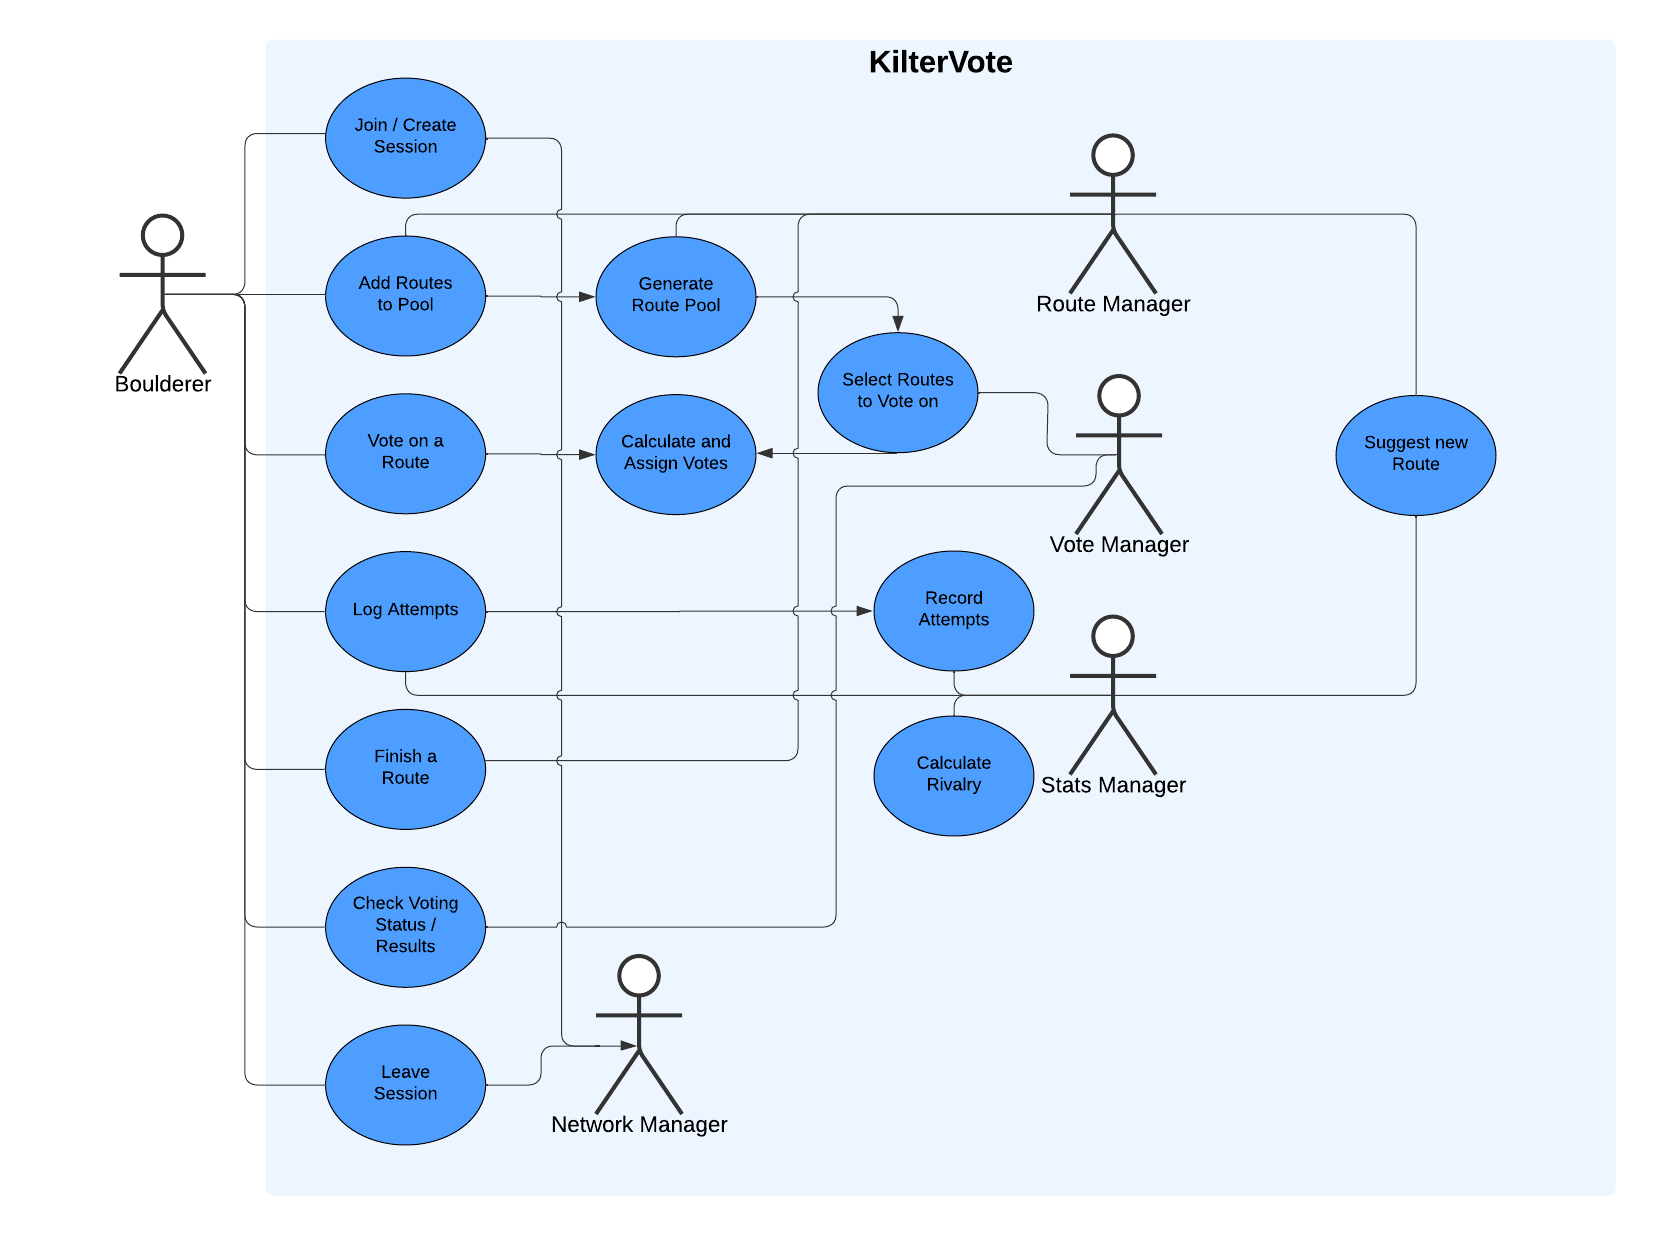
\includegraphics[width=\textwidth]{pictures/Use_Case_Diagram.png}

  \subsection{Wireframes}
    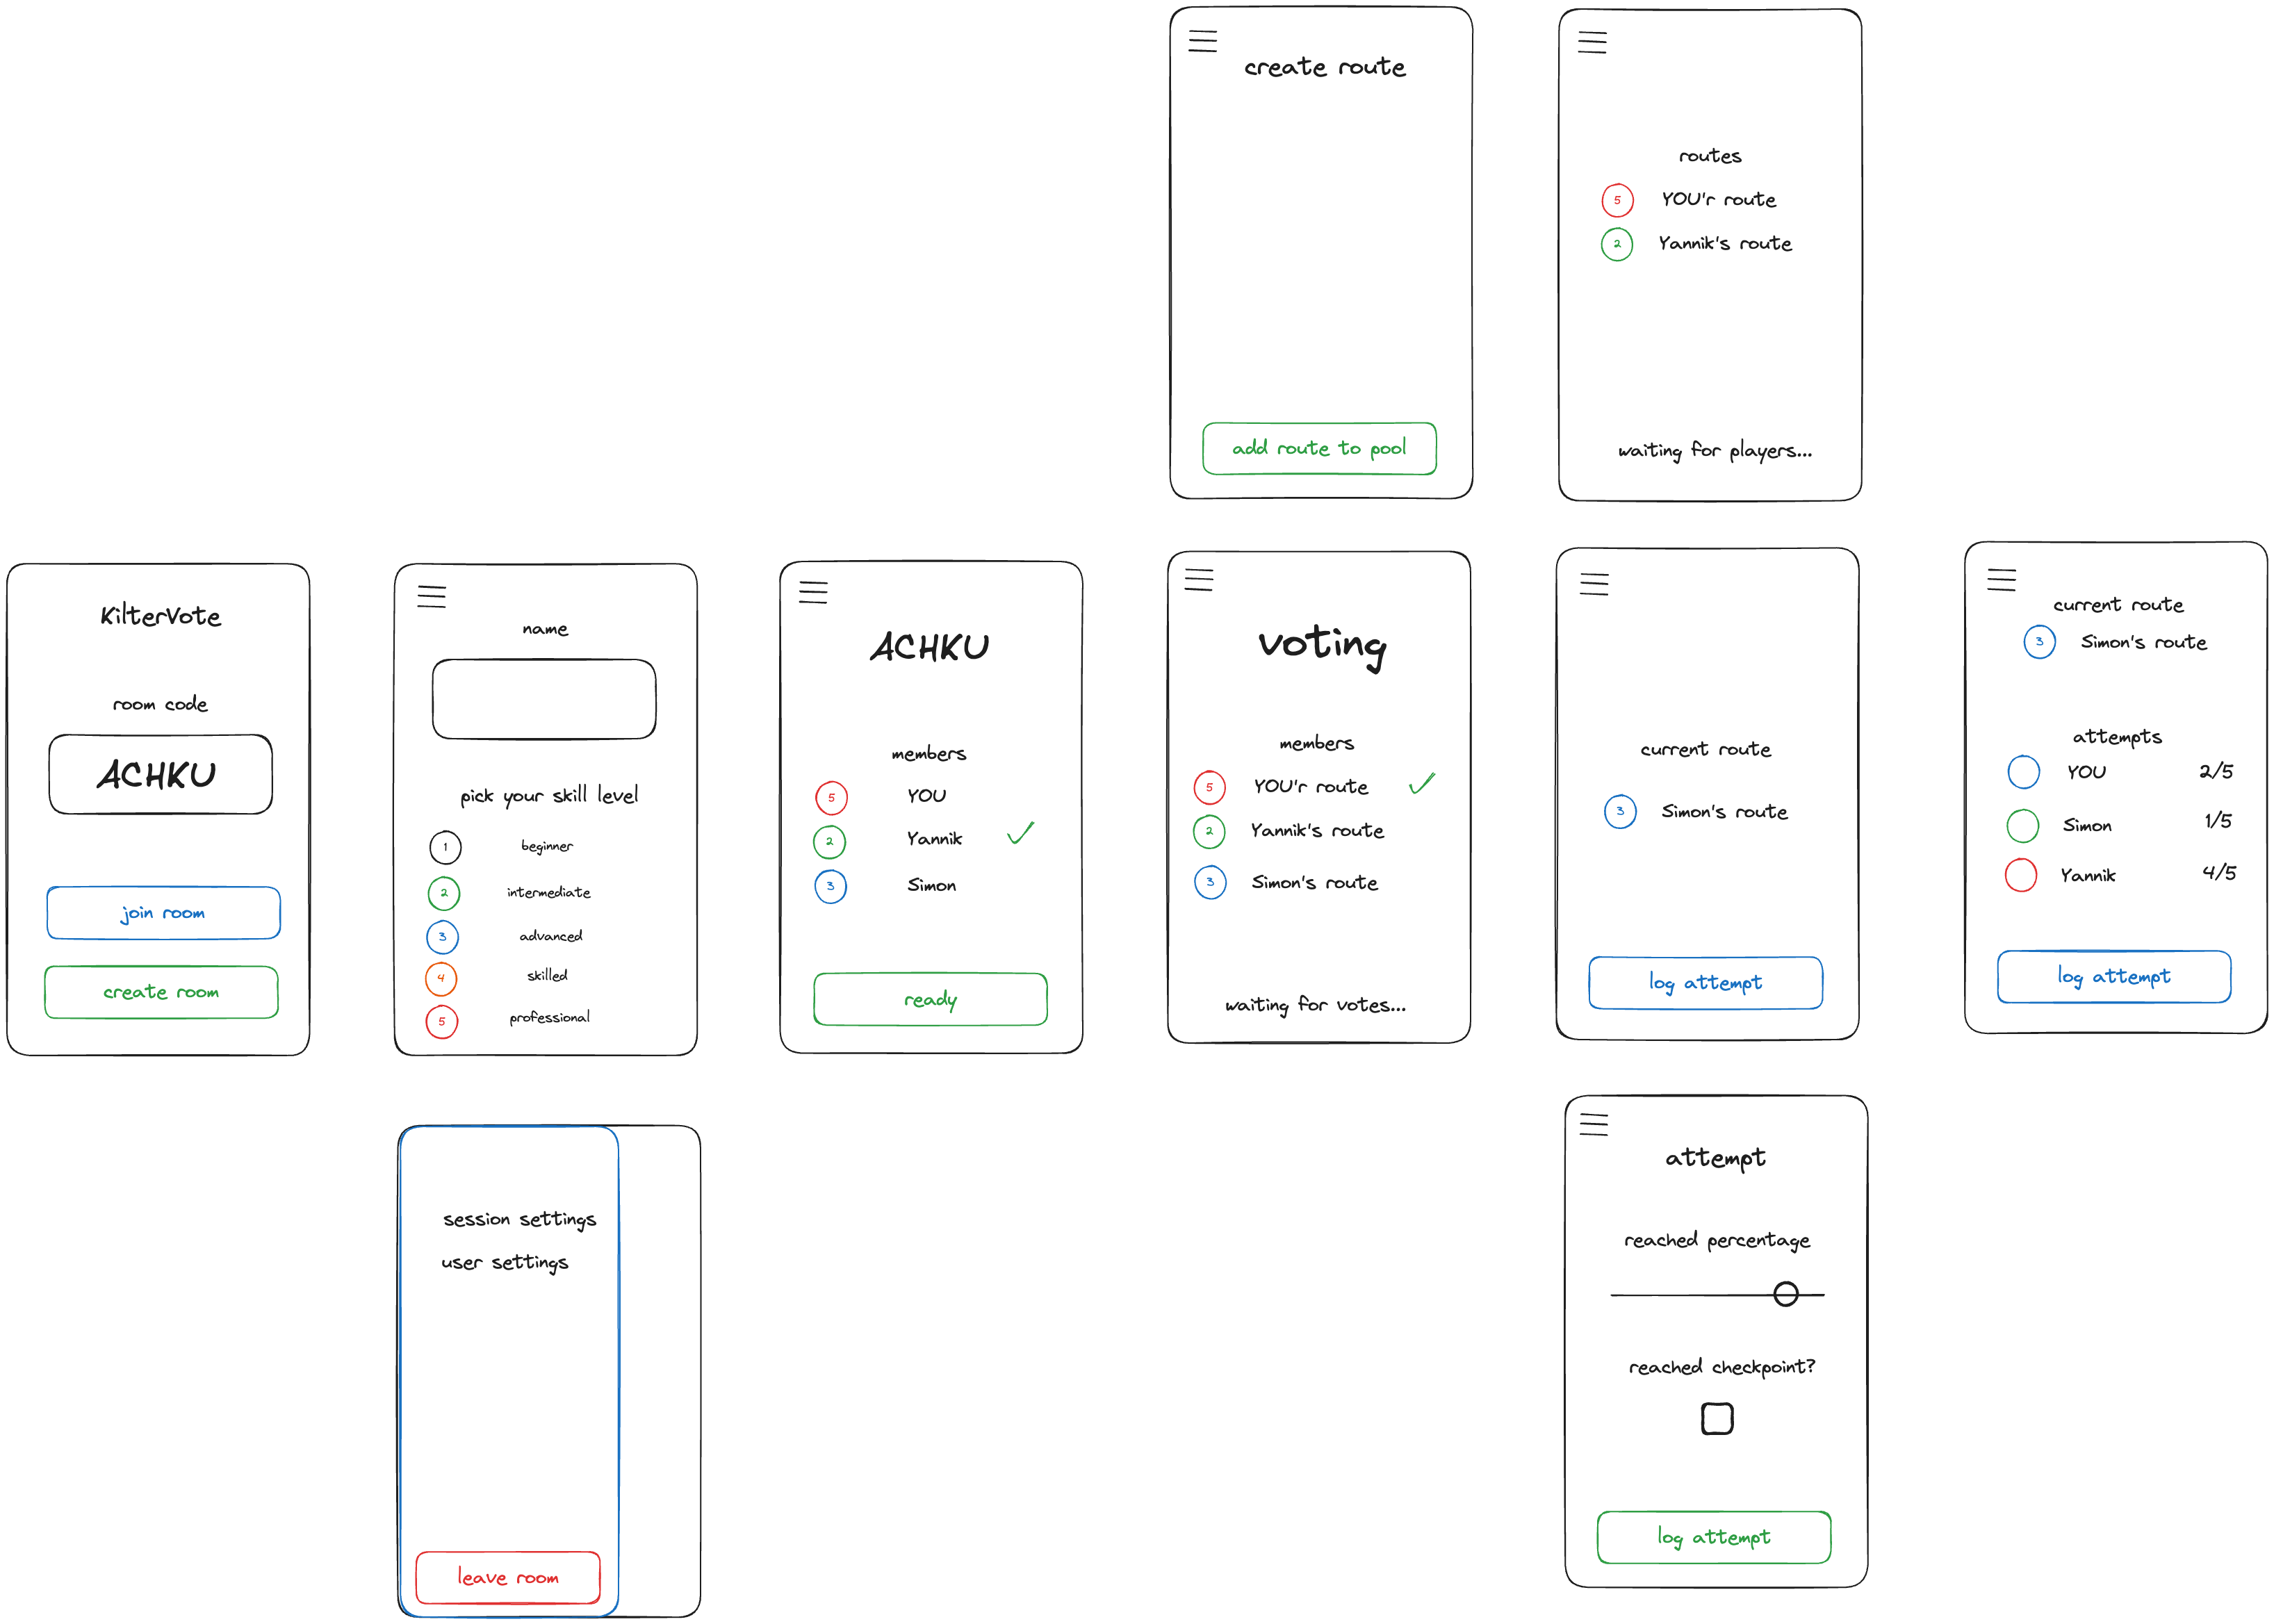
\includegraphics[width=\textwidth]{pictures/KilterVote_GUI.png}

  \subsection{Einordnung in die Anforderungen}  
    \par  
      Die Applikation basiert auf einem Ad-hoc Netzwerk welches zwischen den Geräten der Boulderer aufgebaut wird.
      Dafür ziehen wir Bluetooth, sowie WiFi-Direct in Betracht, im Optimalfall wird die Möglichkeit für beides geboten.
      Die Statistiken der Boulderer und die Versuche während der Sessions werden auf dem persönlichen Gerät gespeichert und dann im Ad-hoc Netzwerk gepublished, somit liegen die Daten immer verteilt auf mehreren Geräten.
      Lässt es der zeitliche Rahmen zu besteht auch die Möglichkeit NFC für das Beitreten/Erstellen einer Session zwischen Boulderern zu nutzen.
    
\newpage

\section{Komponenten}
Komponenten Diagramm:
    \newline
    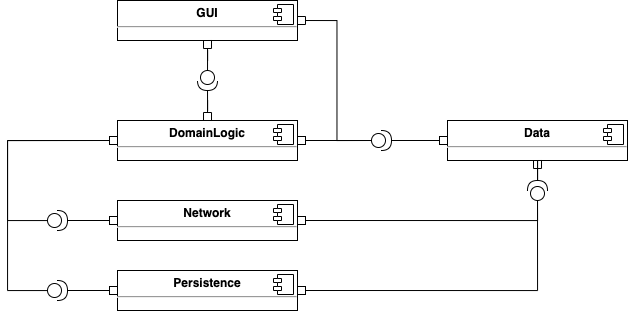
\includegraphics[width=\textwidth]{pictures/component_diagram.drawio.png}

  \par
    Ganz grob besteht die Applikation aus 5 Komponenten.
    \begin{enumerate}
      \item GUI
      \item Data
      \item Domain Logic
      \item Network
      \item Persistence
    \end{enumerate}
    Die GUI Komponente greift dabei auf die Domain Logic Komponente zu, welche die nötigen Daten zur Anzeige in der GUI bereitstellt.
    Die Domain Logic Komponente wiederum greift auf die Network Komponente und die Persistence Komponente zu.
    Über diese beiden Komponenten erfragt die Domain Logic Komponente die nötigen Daten, entweder von anderen Geräten im gleichen Ad-hoc Netzwerk oder durch die auf dem Gerät gespeicherten Daten.
    Alle diese Komponenten greifen auf die Date Komponente zu, da in diesem die Modelle der einzelnen Datenstrukturen liegen.

  \subsection{GUI}
    \par
      Die bereits erwähnten Use Cases, sowie die Wireframes bilden bereits ein gutes Konzept für die GUI.
      Es wird nicht viele Activities geben, was genau auf der GUI angezeigt wird hängt hauptsächlich vom aktuellen Status der Session ab und kann somit durch verschiedene Fragments realisiert werden.
      Die GUI bietet keine Schnittstelle, da sie nur auf andere Komponenten zugreift.
      Das Testen dieser ist nur durch End-to-End Test möglich z.B. durch Bibliotheken wie Espresso.

    \newpage
    \subsubsection{Main Activity}

      \subsubsubsection{Sessions}
        \par
          Ist der Boulderer noch keiner Session beigetreten, kann er dies im Hauptbildschirm tun oder eine neue erstellen.
          Ist die Session erstellt werden alle beigetretenen Boulderern mit Namen und Erfahrungslevel angezeigt.
          Hier kann nun ausgewählt werden ob die Boulderer ihre Statistiken vergleichen wollen oder eine Kilter Runde starten wollen.

      \subsubsubsection{Rivalitäten}
        \par
          Jeder Boulderer published seine eigenen Statistiken im bestehenden Ad-hoc Netzwerk, so können Statistiken angezeigt und untereinander verglichen werden.

      \subsubsubsection{RoutePool}
        \par
          Sind alle Boulderer bereit beginnen die Boulderer mit dem Befüllen des Routen Pools.
          Hierzu können sie entweder bereits erstellte Route auswählen, oder komplett neue Routen erstellen.

      \subsubsubsection{Voting}
        \par
          Ist dieser befüllt, können die Boulderer für eine Route stimmen.
          Haben alle Boulderer ihre Stimme abgegeben, wird eine Route ausgewählt und jeder Boulderer kann mit seinen Versuchen beginnen.

      \subsubsubsection{Attempts}
        \par
          Der Boulderer mit dem aktuellen Versuch bekommt die Möglichkeit seinen Versuch abzuschliessen indem er seinen Fortschritt in Prozenten angibt.
          Das geht so lange bis alle Boulderer die Route geschafft haben oder ihre Versuche verbraucht sind dann können die Boulderer wieder für eine Route abstimmen.

    \subsubsection{Route Creator}
      \par
        In dieser Activity wird den Boulderern die Möglichkeit gegeben eine eigene Route zu erstellen, abzuändern und zu speichern.


  \subsection{Data}
    \par
      Hier liegen wie bereits erwähnt die verschiedenen Models der einzelnen Datenstrukturen.
      Nach aktuellem Stand sind folgende Strukturen von Relevanz:
      \begin{enumerate}
        \item User
        \item Route
        \item Vote
        \item Statistics
      \end{enumerate}

    \subsubsection{User}
      \par
        Der User besteht hauptsächlich aus:
        \begin{itemize}
          \item Name
          \item durchschnittliches Erfahrungslevel
          \item Statistics
        \end{itemize}

    \subsubsection{Route}
      \par
        Eine Route ist charakterisiert durch:
        \begin{itemize}
          \item Schwierigkeitsgrad
          \item Darstellung der Route (wahrscheinlich als Bild, oder in Form eines Arrays)
        \end{itemize}

    \subsubsection{Vote}
      \par
        Ein Vote hat folgende Bestandteile:
        \begin{itemize}
          \item gewählte Route
          \item Gewichtung des Votes
        \end{itemize}

    \subsubsection{Statistics}
      \par
        Nach aktuellem Stand wollen wir vor allem die folgenden Daten in den Statistics unterbringen: 
        \begin{itemize}
          \item höchstes erreichtes Erfahrungslevel
          \item Versuche pro Route inklusive prozentualem Fortschritt auf dieser Route
        \end{itemize}

  \subsection{Domain Logic}
    \par
      Diese Komponente kann völlig unabhängig von Android implementiert werden und eignet sich damit für Unit Tests. Abhängigkeiten von der Network und Persistence Komponente können gemockt werden.
      Aufgabe dieser Komponente ist die Steuerung zwischen Nutzerinteraktionen und dem Bereitstellen der benötigten Daten für die verschiedenen Activities/Fragments.
      Damit werden folgende Aktionen bereitgestellt:
      \begin{itemize}
        \item Session erstellen
        \item Boulderer zu Session hinzufügen
        \item Boulderer von Session entfernen
        \item Routen zum Pool hinzufügen
        \item Routen Pool abfragen
        \item Abstimmen für Routen in Pool
        \item Meist gewählte Route abfragen
      \end{itemize}

  \subsection{Network}
    \par
      Mit dieser Komponente werden die einzelnen Verbindungen zwischen den Geräten der Boulderer hergestellt. Außerdem werden die Anfragen von bestimmten Daten, sowie deren Antworten zwischen den Geräten ausgetauscht.
      Die Network Komponente bietet folgende Funktionen:
      \begin{itemize}
        \item Session erstellen
        \item Session beitreten
        \item Session verlassen
        \item Session Information aktualisieren
      \end{itemize}

  \subsection{Persistence}
    \par
      Diese Komponente übernimmt das Speichern der für den Boulderer relevanten Daten.
      Dazu gehören:
      \begin{itemize}
        \item Boulderer Name
        \item Boulderer Erfahrungslevel
        \item Statistiken des Boulderers pro Route
      \end{itemize}

\section{Interfaces und Testing}
\subsection{Network}
\begin{verbatim}
interface Network {
    fun getNearbySessions(): List<Session>
    fun joinSession(sessionId: String)
    fun leaveSession()
    fun createSession(): Session
    fun updateSessionInfo(sessionDetails: SessionDetails)
}
\end{verbatim}
Unit Tests
 \begin{itemize}
	\item \texttt{getNearbySessions()} gibt Sessions zurück (mit mocked nearby sessions)
	\item \texttt{getNearbySessions()} gibt keine Sessions zurück (ohne nearby sessions)
	\item \texttt{joinSession()} tritt gemockter Session bei
	\item \texttt{leaveSession()} verlässt gemockte Session
	\item \texttt{createSession()} erstellt neue Session
	\item \texttt{updateSessionInfo()} setzt Session Details (testen via Spy)
\end{itemize}

\subsection{Pool} 
\begin{verbatim}
interface Pool {
    fun createPool(): Pool
    fun getPoolDetails(): PoolDetails
}
\end{verbatim}
Unit Tests
\begin{itemize}
	\item \texttt{createPool()} erstellt eine neue Instanz von \texttt{Pool}
	\item \texttt{createPool()} gibt gültige \texttt{Pool}-Daten zurück (z. B. mit gemockter Implementierung prüfen)
	\item \texttt{createPool()} erstellt keine Duplikate, wenn ein Pool bereits existiert (ggf. mit Singleton-Mechanismus testen)
\end{itemize}

\subsection{Statistics} 
\begin{verbatim}
interface Statistics {
    fun setNewHighestGrade(highestGrade: Grade)
    fun setCurrentRouteProgress(progress: Int)
    fun addFinishedRoute(finished: Route)
    fun addRivalryWin(rival: Rival)
}
\end{verbatim}
Unit Tests
\begin{itemize}
	\item \texttt{setNewHighestGrade()} setzt neues Höchstgrad (mit Mock-Datenbank prüfen)
	\item \texttt{setCurrentRouteProgress()} aktualisiert Fortschritt (mit Mock überprüfen)
	\item \texttt{addFinishedRoute()} fügt abgeschlossene Route in Datenbank ein
	\item \texttt{addRivalryWin()} fügt Rivalitätsgewinn in Datenbank ein
\end{itemize}

\subsection{Route} 
\begin{verbatim}
interface Route {
    fun getRouteByName(name: String): Route?
    fun getRoutesByGrade(grade: Grade): List<Route>
}
\end{verbatim}
Unit Tests
\begin{itemize}
	\item \texttt{getRouteByName()} gibt existierende (mock) Route zurück
	\item \texttt{getRouteByName()} gibt \texttt{null} zurück, wenn Route nicht existiert
	\item \texttt{getRoutesByGrade()} gibt Liste der Routen für Grad zurück
	\item \texttt{getRoutesByGrade()} gibt leere Liste zurück, wenn keine Routen existieren
\end{itemize}

\subsection{RouteManager} 
\begin{verbatim}
interface RouteManager {
    fun addVote(vote: Vote)
    fun getWinningRoute(): Route
}
\end{verbatim}
Unit Tests
\begin{itemize}
	\item \texttt{addVote()} fügt Stimme mit hinzu (Stimmengewicht ebenfalls testen)
	\item \texttt{getWinningRoute()} gibt Route mit den meisten Stimmen (unter Berücksichtigung der Gewichtung) zurück
	\item \texttt{getWinningRoute()} gibt \texttt{null}, wenn keine Stimmen vorhanden sind
\end{itemize}

\subsection{Vote} 
\begin{verbatim}
interface Vote {
    fun getRoute(): Route
    fun getVoteWeight(): Int
}
\end{verbatim}
Unit Tests
\begin{itemize}
	\item \texttt{getRoute()} gibt die Route zurück, die abgestimmt wurde
	\item \texttt{getVoteWeight()} gibt korrektes Stimmgewicht zurück
\end{itemize}

\subsection{VoteManager} 
\begin{verbatim}
interface VoteManager {
    fun addRoute(route: Route)
    fun removeRoute(route: Route)
    fun getRoutes(): List<Route>
}
\end{verbatim}
Unit Tests
\begin{itemize}
	\item \texttt{addRoute()} fügt neue Route hinzu
	\item \texttt{getRoutes()} gibt Liste aller hinzugefügten Routen zurück
	\item \texttt{getRoutes()} gibt leere Liste zurück, wenn keine Routen hinzugefügt wurden
\end{itemize}

\newpage

\subsection{Integration Tests}
\begin{table}[h]
\centering
\begin{tabular}{|p{5cm}|p{5cm}|p{5cm}|}
\hline
getestete Komponenten & Test Beschreibung & erwartetes Resultat \\
\hline
\texttt{Network} + \texttt{Pool} & Abhängigkeit zwischen Network und Pool & eine neue Session erstellt auch einen dazugehörigen Pool \\
\hline
\texttt{RouteManager} + \texttt{VoteManager} & einfache Interkation zwischen Route- und VoteManager & eine einzige Wahl auf eine Route führt dazu, dass diese Route die Wahl gewinnt \\
\hline
\texttt{Pool} + \texttt{Statistics} & Highscores und andere Statistiken werden beim Beenden einer Runde gesetzt & gegebene Statistiken sind am ende der Runde in der Datenbank \\
\hline

\end{tabular}
\end{table}

\end{document}
